\documentclass{beamer}%
\usepackage[T1]{fontenc}%
\usepackage[utf8]{inputenc}%
\usepackage{lmodern}%
\usepackage{textcomp}%
\usepackage{lastpage}%
\usepackage{graphicx}%
\usepackage{xcolor}%
\usepackage{tcolorbox}%
%
\title{Yair company}%
\author{Your Name}%
\date{\today}%
\usepackage{booktabs}%
%
\begin{document}%
\normalsize%
\section{Title}%
\label{sec:Title}%
\begin{frame}%
\frametitle{}%
\textbf{Company Name: }%
AURA.TA%
\textbf{ Industry: }%
Construction%


\begin{figure}[h!]%
\centering%

\includegraphics[width=30mm]{company_logo.jpg}%
\end{figure}

%
\end{frame}

%
\section{Introduction}%
\label{sec:Introduction}%
\begin{frame}%
\frametitle{Introduction}%


\begin{figure}[h!]%
\centering%

\includegraphics[width=100mm]{intro.png}%
\end{figure}

%
\end{frame}

%
\section{Financial Ratios}%
\label{sec:FinancialRatios}%
\begin{frame}%
\frametitle{Liquidity Ratios}%
This slide presents the calculated liquidity ratios:%
\begin{itemize}%
\item \textbf{Current Ratio}: 1.35%
\item \textbf{Quick Ratio}: 0.58%
\item \textbf{Immediate Liquidity Ratio}: 0.07%
\item \textbf{Cashflow To Sales Ratio}: -0.54%
\end{itemize}%
\end{frame}%
\begin{frame}%
\frametitle{Profitability Ratios}%
This slide presents the calculated profitability ratios:%
\begin{itemize}%
\item \textbf{Net Profit Margin}: 0.11%
\item \textbf{Operating Profit Margin}: 0.13%
\item \textbf{Ebitda Ratio}: 0.20%
\item \textbf{Return On Equity (Roe)}: 0.13%
\item \textbf{Return On Assets (Roa)}: 0.04%
\end{itemize}%
\end{frame}%
\begin{frame}%
\frametitle{Leverage Ratios}%
This slide presents the calculated leverage ratios:%
\begin{itemize}%
\item \textbf{Leverage Ratio}: 0.18%
\item \textbf{Equity To Assets Ratio}: 0.28%
\end{itemize}%
\end{frame}%
\begin{frame}%
\frametitle{Efficiency Ratios}%
This slide presents the calculated efficiency ratios:%
\begin{itemize}%
\item \textbf{Receivables Ratio}: 0.59%
\item \textbf{Customers Ratio}: 0.79%
\item \textbf{Inventory Ratio}: 1.80%
\item \textbf{Inventory Turnover Ratio}: 0.56%
\item \textbf{Inventory Days}: 685.97%
\item \textbf{Payables Days}: 47.01%
\end{itemize}%
\end{frame}

%
\section{Altman Z{-}Score}%
\label{sec:AltmanZ{-}Score}%
\begin{frame}%
\frametitle{Altman Z-Score}%
Altman Z{-}Score for AURA.TA: 2.29 \newline%
%
\end{frame}

%
\section{RESULTS}%
\label{sec:RESULTS}%
\begin{frame}%
\frametitle{RESULTS}%

    \begin{table}[ht]
    \centering
    \tiny
    \begin{tabular}{lcccccc}
    \toprule
     & \textbf{2023-12-31} & \textbf{2022-12-31} & \textbf{2021-12-31} & \textbf{2020-12-31} \\
    \midrule
    \textbf{Interest Expense} & 51,141,000.0 & 29,603,000.0 & 34,589,000.0 & 50,946,000.0 \\
\textbf{Interest Income} & 2,093,000.0 & 417,000.0 & 1,472,000.0 & 1,109,000.0 \\
\textbf{Net Income} & 117,686,000.0 & 140,538,000.0 & 113,533,000.0 & 42,143,000.0 \\
\textbf{Tax Provision} & 34,590,000.0 & 31,824,000.0 & 30,848,000.0 & 15,046,000.0 \\
\textbf{Pretax Income} & 152,934,000.0 & 172,833,000.0 & 144,382,000.0 & 57,180,000.0 \\
\textbf{Operating Income} & 138,392,000.0 & 123,493,000.0 & 114,002,000.0 & 88,703,000.0 \\
\textbf{Selling And Marketing Expense} & 18,981,000.0 & 19,556,000.0 & 11,306,000.0 & 15,688,000.0 \\
\textbf{General And Administrative Expense} & 8,025,000.0 & 6,518,000.0 & 4,368,000.0 & 4,424,000.0 \\
\textbf{Gross Profit} & 190,983,000.0 & 139,443,000.0 & 137,097,000.0 & 130,336,000.0 \\
\textbf{Cost Of Revenue} & 848,888,000.0 & 709,572,000.0 & 756,793,000.0 & 975,039,000.0 \\
\textbf{Total Revenue} & 1,039,871,000.0 & 849,015,000.0 & 893,890,000.0 & 1,105,375,000.0 \\

    \bottomrule
    \end{tabular}
    \caption{Financial Data from 2023 to 2019}
    \label{tab:financial_data}
    \end{table}
    %
\end{frame}

%
\section{Vertical}%
\label{sec:Vertical}%
\begin{frame}%
\frametitle{Vertical}%

    \begin{table}[ht]
    \centering
    \tiny
    \begin{tabular}{lcccccc}
    \toprule
     & \textbf{2023-12-31} & \textbf{2022-12-31} & \textbf{2021-12-31} & \textbf{2020-12-31} \\
    \midrule
    \textbf{Interest Expense} & 4.92\% & 3.49\% & 3.87\% & 4.61\% \\
\textbf{Interest Income} & 0.20\% & 0.05\% & 0.16\% & 0.10\% \\
\textbf{Net Income} & 11.32\% & 16.55\% & 12.70\% & 3.81\% \\
\textbf{Tax Provision} & 3.33\% & 3.75\% & 3.45\% & 1.36\% \\
\textbf{Pretax Income} & 14.71\% & 20.36\% & 16.15\% & 5.17\% \\
\textbf{Operating Income} & 13.31\% & 14.55\% & 12.75\% & 8.02\% \\
\textbf{Selling And Marketing Expense} & 1.83\% & 2.30\% & 1.26\% & 1.42\% \\
\textbf{General And Administrative Expense} & 0.77\% & 0.77\% & 0.49\% & 0.40\% \\
\textbf{Gross Profit} & 18.37\% & 16.42\% & 15.34\% & 11.79\% \\
\textbf{Cost Of Revenue} & 81.63\% & 83.58\% & 84.66\% & 88.21\% \\
\textbf{Total Revenue} & 100.00\% & 100.00\% & 100.00\% & 100.00\% \\

    \bottomrule
    \end{tabular}
    \caption{Vertical Analysis of Financial Data from 2023 to 2019}
    \label{tab:vertical_data}
    \end{table}
    %
\end{frame}

%
\section{Analysis}%
\label{sec:Analysis}%
\begin{frame}%
\frametitle{Analysis}%


\begin{figure}[h!]%
\centering%

\includegraphics[width=80mm]{Ratios_Anlysis.png}%
\end{figure}

%
\end{frame}

%
\section{Directorial Report}%
\label{sec:DirectorialReport}%
\begin{frame}%
\frametitle{Directorial Report}%


\begin{figure}[h!]%
\centering%

\includegraphics[width=80mm]{Directorion.png}%
\end{figure}

%
\end{frame}

%
\section{Market Capitalization}%
\label{sec:MarketCapitalization}%
\begin{frame}%
\frametitle{Conclusions}%


\begin{figure}[h!]%
\centering%
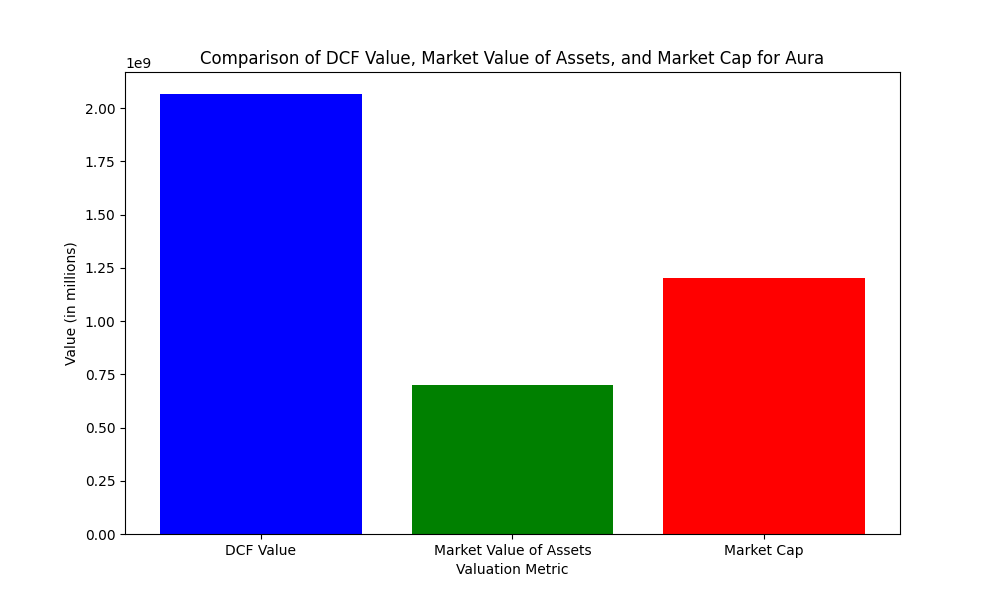
\includegraphics[width=80mm]{valuation_comparison.png}%
\end{figure}

%
\end{frame}

%
\end{document}